\chapter{Experiment and Result}
brief of experiment and result.
\section{Experiment}
Please tell how the experiment conducted from method.

\section{Result}
Please provide the result of experiment

\section{Ahmad Syafrizal Huda/1164062}
\subsection{Teori}
\begin{enumerate}
\item Klasifikasi teks adalah proses pemberian kategori ke dalam teks/dokumen sesuai dengan tipikal dalam supervised machine
\par learning (ML) yang bisa berupa buku perpustakaan, halaman web, artikel media, galeri, dan lain sebagainya. Tujuannya 
\par untuk memberikan label pada setiap teks/dokumen.
\par Contoh ilustrasi gambar dapat dilihat pada gambar \ref{c4_1}
\begin{figure}[ht]
	\centerline{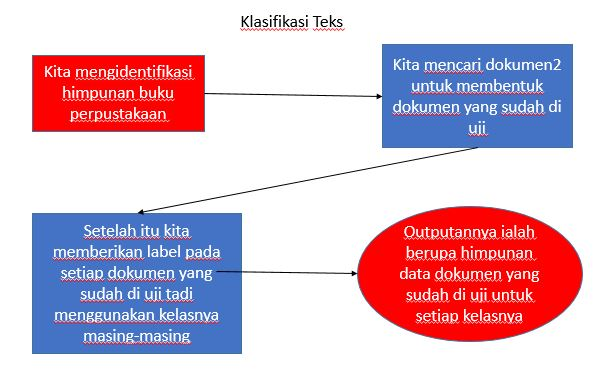
\includegraphics[width=1\textwidth]{figures/huda/chapter4/1.JPG}}
	\caption{Klasifikasi Teks}
	\label{c4_1}
\end{figure}
\item Mengapa klasifikasi bunga tidak dapat menggunakan machine learning? itu dikarenakan memiliki masalah masukan(input) 
\par yang sama tetapi keluarannya (output) yang berbeda, biasanya output yang berbeda ini disebut dengan istilah 'noise'.
\par Noise berarti output yang disimpan bukan seperti seharusnya ( keluaran yang tidak diinginkan ). 
\par Contoh ilustrasi gambar dapat dilihat pada gambar \ref{c4_2}
\begin{figure}[ht]
	\centerline{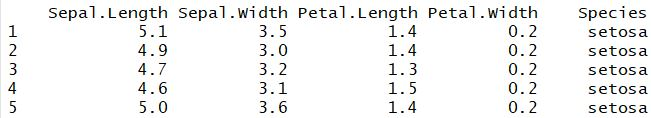
\includegraphics[width=1\textwidth]{figures/huda/chapter4/2.JPG}}
	\caption{Klasifikasi Bunga}
	\label{c4_2}
\end{figure}
\item Teknik pembelajaran mesin pada teks biasanya menggunakan teknik bag-of-words pada klasifikasi berbasis text dan kata 
\par untuk mengklasifikasikan komentar yang ada diinternet sebagai spam atau bukan. Misalkan pada kolom komentar di youtube
\par dapat di cek seberapa sering suatu kata muncul dalam kalimat. Setiap kata dapat dijadikan baris dan kolomn yang 
\par merupakan kategori kata tersebut, apakah masuk kedalam spam atau tidak. dan contoh lainnya yaitu pada Caption. dimana
\par akan muncul subtitle secara otomatis dari youtube menggunakan sensor suara yang disesuaikan dengan kata yang telah 
\par ditentukan. 
\par Contoh ilustrasi gambar dapat dilihat pada gambar \ref{c4_3}
\begin{figure}[ht]
	\centerline{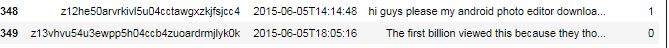
\includegraphics[width=1\textwidth]{figures/huda/chapter4/3.JPG}}
	\caption{Comment Youtube}
	\label{c4_3}
\end{figure}
\item Vektorisasi data merupakan pembagian dan pemecahan data yang kemudian nantinya data tersebut akan menjadi beberapa data
\par Contoh misalkan dari sebuah paragraph nantinya kan di pecah menjadi beberapa kalimat dari kalimat tersebut dibagi lagi
\par menjadi beberapa kata.
\item Bag-of-words adalah cara untuk merepresentasikan data teks saat memodelkan teks yang menggambarkan kemunculan 
\par kata-kata dalam dokumen dengan algoritma pembelajaran mesin.
\par Contoh ilustrasi gambar dapat dilihat pada gambar \ref{c4_4}
\begin{figure}[ht]
	\centerline{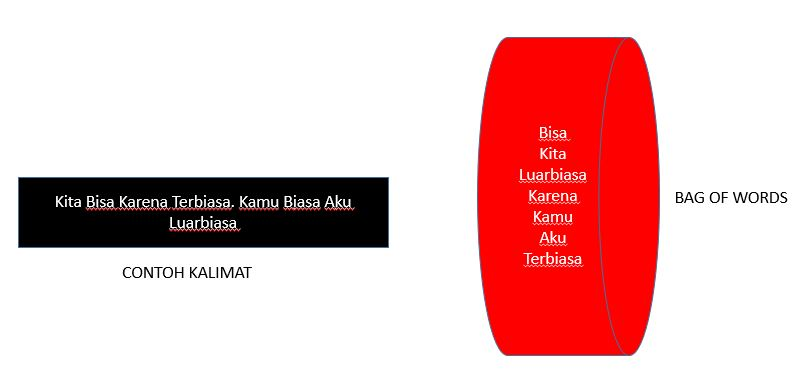
\includegraphics[width=1\textwidth]{figures/huda/chapter4/4.JPG}}
	\caption{Bag Of Words}
	\label{c4_4}
\end{figure}
\item TF-IDF  memberi kita frekuensi kata dalam setiap dokumen atau mengganti data jadi number. Ini adalah rasio berapa 
\par kali kata itu muncul dalam dokumen dibandingkan dengan jumlah total kata dalam dokumen itu. Itu meningkat seiring 
\par jumlah kemunculan kata itu di dalam dokumen meningkat. Setiap dokumen memiliki tf sendiri.
\par Contoh ilustrasi gambar dapat dilihat pada gambar \ref{c4_5}
\begin{figure}[ht]
	\centerline{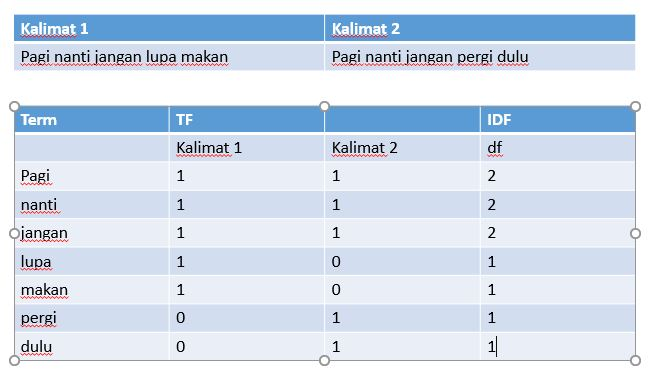
\includegraphics[width=1\textwidth]{figures/huda/chapter4/5.JPG}}
	\caption{TF-IDF}
	\label{c4_5}
\end{figure}
\end{enumerate}

\subsection{Praktek Program}
\begin{enumerate}
\item Kali ini kita akan membuat data dummy dengan format csv di sini saya mengambil data dari web UCI Machine Learning 
\par Repository dengan nama file Holiday.csv seperti pada gambar \ref{c4_6}
\begin{figure}[ht]
	\centerline{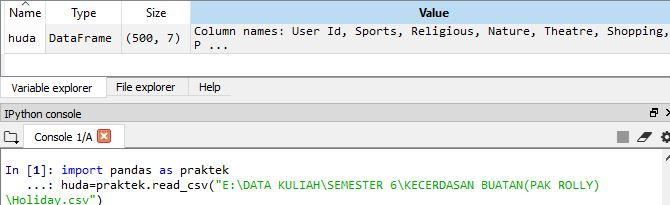
\includegraphics[width=1\textwidth]{figures/huda/chapter4/6.JPG}}
	\caption{Data Dummy 500 Data}
	\label{c4_6}
\end{figure}
\subitem Pada codingan \ref{c4_6} yaitu mengimport librari pandas dimana kita mengaliaskan praktek sebagai pandas. Pandas berguna untuk mengelola  dataframe = matrix = tabel kemudian memanggil nama alias untuk membaca format csvnya.
\item Dari dataframe yang sudah ada sebelumnya kita akan membagi menjadi 2 yaitu 450 row pertama dan 50 row sisanya dapat
\par dilihat pada gambar \ref{c4_7}
\begin{figure}[ht]
	\centerline{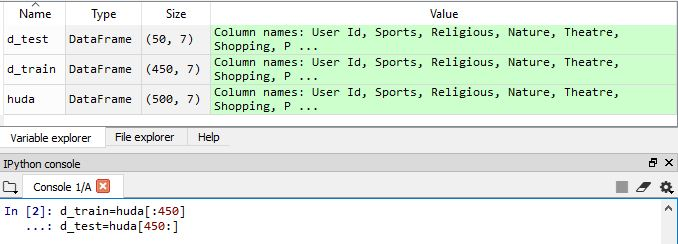
\includegraphics[width=1\textwidth]{figures/huda/chapter4/7.JPG}}
	\caption{Membagi 2 Dataframe}
	\label{c4_7}
\end{figure}
\subitem Pada codingan \ref{c4_7} yaitu baris pertama dimana d\_train untuk membagi data training sebanyak 450 row dan pada 
\par baris kedua dimana d\_test untuk data sisa atau data yang baru sebanyak 50 row.
\item Melakukan Vektorisasi dan Klasifikasi Data pada data Eminem pada gambar \ref{c4_8} huda merupakan dataframe keseluruhan dari file csv yang sudah dimasukkan dengan jumlah 448 baris dan 5 kolom. nospam merupakan dataframe yang isinya hanya data yang bukan termasuk spam dengan inisial angka 0. Sedangkan spam merupakan dataframe yang isinya hanya data spam dengan inisial angka 1.
\begin{figure}[ht]
	\centerline{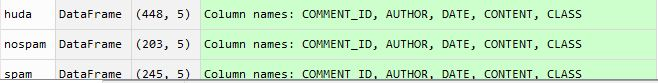
\includegraphics[width=1\textwidth]{figures/huda/chapter4/8.JPG}}
	\caption{Vektorisasi dan Klasifikasi Data}
	\label{c4_8}
\end{figure}
\subitem  Pada gambar \ref{c4_9} merupakan hasil output content dimana terdapat 448 baris/data yang mempunyai 1602 kata-kata \par yang digunakan pada komentar yang ada di content tersebut.
\begin{figure}[ht]
	\centerline{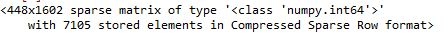
\includegraphics[width=1\textwidth]{figures/huda/chapter4/9.JPG}}
	\caption{Data Content}
	\label{c4_9}
\end{figure}
\subitem Pada gambar \ref{c4_10} maksud dari outputannya merupakan dataframe kata-kata tadi yang berjumlah 1602 kata orang \par yang komen pada data eminem.
\begin{figure}[ht]
	\centerline{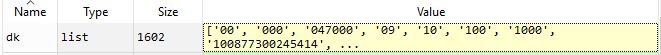
\includegraphics[width=1\textwidth]{figures/huda/chapter4/10.JPG}}
	\caption{DataFrame Kata-kata Pada Content}
	\label{c4_10}
\end{figure}
\item Mengklasifikasikan dari data vektorisasi dengan menggunakan klasifikasi svm(support vektorisasi machine) dapat dilihat pada \par gambar \ref{c4_11}.
\begin{figure}[ht]
	\centerline{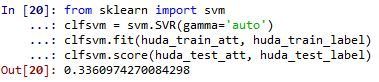
\includegraphics[width=1\textwidth]{figures/huda/chapter4/11.JPG}}
	\caption{Klasifikasi SVM Dari Data Vektorisasi}
	\label{c4_11}
\end{figure}
\subitem Jadi pada gambar \ref{c4_11} merupakan hasil dari memprediksi data score vektorisasi dengan svm menggunakan metode \par fit dimana digunakan untuk data training atau data pelatihannya saja.
\item Mengklasifikasikan dari data vektorisasi dengan menggunakan klasifikasi Decision Tree dapat dilihat pada gambar \ref{c4_12}.
\begin{figure}[ht]
	\centerline{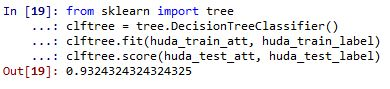
\includegraphics[width=1\textwidth]{figures/huda/chapter4/12.JPG}}
	\caption{Klasifikasi Decision Tree Dari Data Vektorisasi}
	\label{c4_12}
\end{figure}
\subitem Jadi pada gambar \ref{c4_12} merupakan hasil dari memprediksi data score vektorisasi dengan Decision Tree menggunakan \par metode fit dimana digunakan untuk data training atau data pelatihannya saja.
\item Mengeplot confusion matrix menggunakan matplotlib dapat dilihat pada gambar \ref{c4_13}.
\begin{figure}[ht]
	\centerline{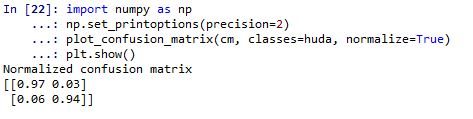
\includegraphics[width=1\textwidth]{figures/huda/chapter4/13.JPG}}
	\caption{Plot Confusion Matrix Menggunakan Matplotlib}
	\label{c4_13}
\end{figure}
\subitem Pada gambar \ref{c4_13} sebelumnya kita harus mengimport matplotlibnya terlebih dahulu setelah itu di sini saya 
\par menggunakan numpy untuk mengeluarkan hasil plot confusion matrix pada matplolibnya nantinya akan keluar normalisasi dari \par confusion matrix berupa data baris dan kolom. 
\item Menjalankan program cross validation pada data vektorisasi dapat dilihat pada gambar \ref{c4_14}.
\begin{figure}[ht]
	\centerline{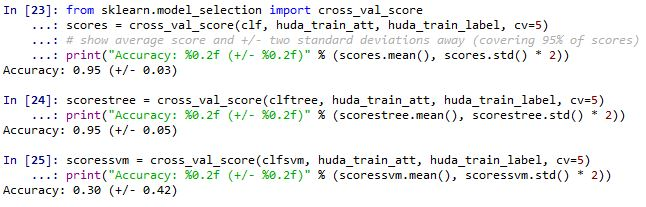
\includegraphics[width=1\textwidth]{figures/huda/chapter4/14.JPG}}
	\caption{Program Cross Validation Pada Data Vektorisasi}
	\label{c4_14}
\end{figure}
\subitem Pada gambar\ref{c4_14} yang pertama yaitu memunculkan akurasi cross validation dari random forest pada data yang sudah divektorisasi, yang kedua yaitu memunculkan akurasi cross validation dari decision tree pada data yang sudah divektorisasi, dan yang ketiga yaitu memunculkan akurasi cross validation dari svm pada data yang sudah divektorisasi.
\item Membuat program pengamatan komponen informasi pada data yang sudah divektorisasi dapat dilihat pada gambar \ref{c4_15}.
\begin{figure}[ht]
	\centerline{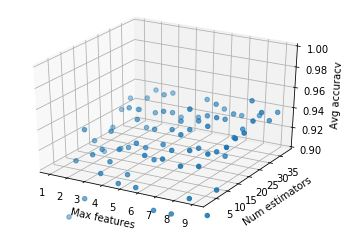
\includegraphics[width=1\textwidth]{figures/huda/chapter4/15.JPG}}
	\caption{Program Pengamatan Komponen Informasi}
	\label{c4_15}
\end{figure}
\subitem Pada gambar \ref{c4_15} merupakan hasil outputan yang mana max features di sana terdapat 9 data dari 10 yang sudah kita masukkan ke dalam codingan sebelumnya dan penomoran estimatornya merupakan data per 5 dari angka 40 sedangkan rata-rata akurasinya kita tuliskan datanya mulai dari 0.9 sampai dengan 1. Titik-titik yang didalam tersebut merupakan data vektorisasi dari pengamatan komponen informasinya.
\end{enumerate}

\subsection{Penanganan Eror}
\begin{enumerate}
\item Pada gambar \ref{c4_16} merupakan ScreeShootan dari data yang eror.
\begin{figure}[ht]
	\centerline{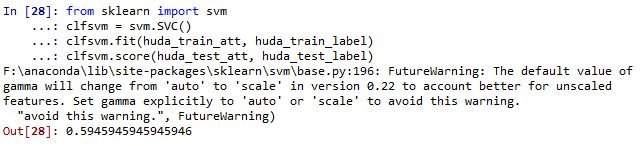
\includegraphics[width=1\textwidth]{figures/huda/chapter4/eror.JPG}}
	\caption{Eror Pada Coding SVM}
	\label{c4_16}
\end{figure}
\item 
\begin{verbatim}
 clfsvm = svm.SVC()
F:\anaconda\lib\site-packages\sklearn\svm\base.py:196: FutureWarning: The default value of gamma will change from 'auto' to 'scale' in version 0.22 to account better for unscaled features. Set gamma explicitly to 'auto' or 'scale' to avoid this warning.
  "avoid this warning.", FutureWarning)
\end{verbatim}
\item Solusi pemecah masalah eror tersebut dengan mengganti dan menambahkan codingan tersebut seperti berikut.
\begin{verbatim}
from sklearn import svm
clfsvm = svm.SVR(gamma='auto')
clfsvm.fit(huda_train_att, huda_train_label)
clfsvm.score(huda_test_att, huda_test_label)
\end{verbatim}
\end{enumerate}